\documentclass[a4paper,12pt]{scrreprt}
    %% Used for changing geometry of the page
    %% Cover page text cannot overlay cover sketching/style 
    %% https://ctan.org/pkg/geometry?lang=en
\usepackage{geometry}
    %% Changes language of some packages protocols
    %% e.g., when captioning images: Figure 1. -> Figura 1.
    %% https://ctan.org/pkg/babel?lang=en
\usepackage[portuguese]{babel}
    %% Used for special fonts
    %% Cannot be compiled with pdflatex
    %% https://ctan.org/pkg/fontspec?lang=en
\usepackage{fontspec}
    %% Arial FONT
    \setmainfont{Arial}
\usepackage{subfiles}
    %% More colors and color options
    %% https://ctan.org/pkg/xcolor?lang=en
    %% https://ctan.org/pkg/colortbl?lang=en
\usepackage{xcolor,colortbl}
    %% More tabular options, like dashed/dotted lines
    %% https://ctan.org/pkg/arydshln?lang=en
\usepackage{arydshln}
    %% List of acronyms
    %% https://ctan.org/pkg/nomencl?lang=en
\usepackage[intoc]{nomencl}
    %% Must be called to init nomencl environment  
    \makenomenclature
    %% More images options/settings
    %% https://ctan.org/pkg/graphicx?lang=en
\usepackage{graphics}
    %% Defining subdirectories to image path enviornment
    %% \graphicspath{{sub1}{sub2}...{subN}}
    \graphicspath{{images}}
    
    %% used to handle cross-referencing commands in LaTeX to produce hypertext links in the document
    %% https://ctan.org/pkg/hyperref?lang=en
\usepackage{hyperref}
    %% math environments
    %% https://ctan.org/pkg/amsmath?lang=en

    %% settings
    \hypersetup{
        colorlinks,
        citecolor=black,
        filecolor=black,
        linkcolor=black,
        urlcolor=black
    }

\usepackage{amsmath}
    %% Defining backgrouns, used to make the cover
    %% https://ctan.org/pkg/background?lang=en
\usepackage[some]{background}
    %% Used to make drawings or complex graphics
    %% http://pgf.sourceforge.net/pgf_CVS.pdf
\usepackage{tikz}
    %% Tikz library to point operations ((x1,y1) + (x2,y2))
    \usetikzlibrary{calc}

%% Defining sfdefault font and default font for document
\renewcommand{\familydefault}{\sfdefault}


%% Costume made cover 
%% From there you can use \makecover command to build the cover
%% Blue cover color
\definecolor{titlepagecolor}{RGB}{54,95,145}

%==========================================================================
% COLORED BAR ON THE LEFT SIDE
%==========================================================================

\backgroundsetup{
    scale=1,
    angle=0,
    opacity=1,
    contents={
            \begin{tikzpicture}[remember picture,overlay]
                \path [fill=titlepagecolor]
                (current page.north west) -- ($(current page.north west) + (5,0)$)
                -- ($(current page.south west) + (5,0)$)-- (current page.south west);
                \node[color=white] at ($(current page.south west) + (3,4)$) {\bfseries {\fontsize{50}{60} \textsf{DSS}}};
                %\node[color=titlepagecolor] at ($(current page.south west) + (5.8,4)$) {\bfseries {\fontsize{120}{60} \textsf{4}}};
            \end{tikzpicture}
        }
}

%==========================================================================
% TITLE PAGE INFO
%==========================================================================

%% Changes values in this field to show information in the cover and back cover about your team/project


%% TITLE
\title{Sistema de apoio a departamento técnico}

%% AUTHORS
\author{
    \begin{tabular} { c c }
        
\includegraphics[scale=0.2]{author/marco.jpg} & 
\includegraphics[scale=0.2]{author/marco.jpg} \\
        62608 - Marco Sousa                           & 93198 - Mariana Marques                       \\
        %\hline                                                                                        \\
        
\includegraphics[scale=0.2]{author/marco.jpg} & 
\includegraphics[scale=0.2]{author/miguel.jpg} \\
        93271 - José Malheiro                         & 94269 - Miguel Fernandes
    \end{tabular}
}

%% Date

\date{\today}

%% Course
\newcommand{\Course}{Licenciatura em Engenharia Informática}

%% Department
\newcommand{\Department}{Escola de Engenharia}

%% UniName
\newcommand{\UniName}{Universidade do Minho}

\newcommand{\UcName}{Desenvolvimento de Sistemas de Software}

\newcommand{\GroupId}{Grupo 31}

%% UniPic
\newcommand{\UniPic}{
\includegraphics[scale=0.09]{uminho.png}}

%% University 
\newcommand{\University}{
    \begin{flushleft}
        \UniPic
    \end{flushleft}
    \textcolor{gray}{\small\textbf{\textsf{\UniName}}}\par
    \textcolor{gray!80!white}{\small{\textsf{\Department}}}\par
    \textcolor{gray!70!white}{\small{\textsf{\Course}}}
}

%% UC
\newcommand{\UC}{
    \begin{flushleft}
        \par\textcolor{titlepagecolor}{  \LARGE\textbf{\textsf{Unidade Curricular de \\ \UcName}}}
    \end{flushleft}
}

%% School Year
\newcommand{\SchoolYear}{
    \small{\textsf{Ano Letivo de 2021/2022}}}


%% Define new command to show title, author and date
\makeatletter
\let\Title\@title
\let\Author\@author
\let\Date\@date
\makeatother

%==========================================================================
% CLASSIFICATION SECTION 
%==========================================================================

%% School Year
\newcommand{\ReceptionDate}{}
%% Responsible
\newcommand{\Responsible}{}
%% Evaluation
\newcommand{\Evaluation}{}
%% Observations
\newcommand{\Observations}{}





%% MAKETEMPLATE
\newcommand{\makecover}{

    %==========================================================================
    % BEGIN COVER PAGE 
    %==========================================================================

    %% Removes page number on footer
    \thispagestyle{empty}

    %% No indentation 
    \setlength{\parindent}{0em}

    %% Put Background defined on \backgroundsetup, in this page
    \BgThispage

    %% Changing geometry to prevent overlay with text
    %% At the end of back cover, geometry is default with \restoregeometry
    \newgeometry{top=3.5cm,left=6cm,right=3cm,bottom=2cm}

    %% builds university info defined previously
    \University
    \vspace{1cm}
    %% builds curricular unity info defined previously
    \UC
    %% builds school year info defined previously
    \SchoolYear

    \vspace*{4cm}
    %% bigger space (i think its the default one) between paragraphs 
    \setlength{\parskip}{1em}

    %% builds title info defined previously
    \par\textbf{\textsf{\huge\Title}}
    \par\textbf{\GroupId}
    \vspace{1cm}
    %% builds author(s) info defined previously
    \par\begin{center}
        \Author
    \end{center}

    \vspace{0.5cm}

    %% builds date info defined previously
    \par\Date
    \restoregeometry
    \pagebreak

    %==========================================================================
    % END COVER PAGE 
    %==========================================================================

    %==========================================================================
    % BEGIN BACK COVER PAGE 
    %==========================================================================

    %% Removes page number on footer
    % \thispagestyle{empty}

    % % Changing look of lines in tabular environment 
    % % Dashed -> dotted 
    % %% length of dashes
    % \setlength\dashlinedash{0.3pt}
    % %% space between dashes
    % \setlength\dashlinegap{1.5pt}
    % %% width of dashes
    % \setlength\arrayrulewidth{1.1pt}


    % %% This values can be changed in the preamble
    % \begin{flushright}
    %     \begin{tabular}{ :p{4cm}:p{4cm}: }
    %         \hdashline
    %         Data de Receção & \ReceptionDate \\ [2ex]
    %         \hdashline
    %         Responsável     & \Responsible   \\ [2ex]
    %         \hdashline
    %         Avalição        & \Evaluation    \\ [2ex]
    %         \hdashline
    %         Observações     & \Observations  \\ [7ex]
    %         \hdashline
    %     \end{tabular}
    % \end{flushright}


    % \vspace{10cm}
    % \begin{flushleft}

    %     %% builds title info defined previously
    %     \par\textbf{\textsf{\huge\Title}}
    %     \vspace{1cm}
    %     %% builds author info defined previously
    %     \par\Author

    %     \vspace{0.5cm}

    %     %% builds date info defined previously
    %     \par\Date
    % \end{flushleft}

    % \pagebreak
    %==========================================================================
    % END BACK COVER PAGE 
    %==========================================================================
}


\graphicspath{ {./assets/} }

% TODO
% ABSTRACT - inclui objetivos e descrição MARCO
% abordar motivo de criar passos e material
% considerações finais

\begin{document}

\pagenumbering{gobble}

% builds the cover
\makecover

%==========================================================================
% BEGIN ABSTRACT PAGE
%==========================================================================



%% Abstract name: \Large font size, flushed left and paragraph skip before abstract content
\renewenvironment{abstract}
{\par\noindent\textbf{\Large\abstractname}\par\bigskip}
{}

\begin{flushleft}
    \begin{abstract}
        <<O resumo tem como objectivo descrever de forma sucinta o trabalho realizado. Deverá conter uma pequena introdução, seguida por uma breve descrição do trabalho realizado e terminando com uma indicação sumária do seu estado final. Não deverá exceder as 400 palavras.>> 
        \par \textbf{Área de Aplicação}: <<Identificação da Área de trabalho. Por exemplo: Desenho e arquitectura de Sistemas de Bases de Dados.>> 
        \par \textbf{Palavras-Chave}: <<Conjunto de palavras-chave que permitirão referenciar domínios de conhecimento, tecnologias, estratégias, etc., directa ou indirectamente referidos no relatório. Por exemplo: Bases de Dados Relacionais, Gestão de Índices, JAVA, Protocolos de Comunicação.>>
    \end{abstract}
\end{flushleft}


\pagebreak

%==========================================================================
% END ABSTRACT PAGE 
%==========================================================================

%==========================================================================
% BEGIN INDEXES PAGES
%==========================================================================

%% Changes table of content name
%% Portuguese babel default : "Conteúdo"
%% Personally I prefer "índice"
\renewcommand{\contentsname}{Índice}

\tableofcontents

\pagebreak

\listoffigures

\pagebreak

\listoftables

\pagebreak

%==========================================================================
% END INDEXES PAGES 
%==========================================================================


%==========================================================================
% BEGIN INTRODUCTION
%==========================================================================

%% Starting page numbering here
\pagenumbering{arabic}

\chapter{Introdução}
O presente relatório foi desenvolvido no âmbito da Unidade Curricular (UC) de Desenvolvimento de Sistemas de Software (DSS),
tendo como principal objetivo apresentar uma possível conceção de um Sistema de Gestão para Centros de Reparação de Equipamentos Eletrónicos, doravante designado \textit{aplicação}.

\section{Contextualização}
A procura por um serviço de reparação, compreende um atendimento célere e garantia de acompanhamento ao longo de todo o processo.
Para que tal seja possível, foi proposto pela equipa docente o desenvolvimento de uma aplicação que permita essa gestão.

Desta forma, foi apresentado um conjunto de possíveis cenários de utilização que a aplicação deverá ser capaz de suportar,
dos quais se efetuou um levantamento de requisitos através de estratégias de modelação lecionadas na UC de DSS.

\section{Breve descrição do enunciado proposto}

Tal como referido, o enunciado propõe a conceção e implementação de uma aplicação e apresenta os cenários de utilização que deverão ser
suportados por esta.

Para a fase a que este relatório se refere - \textbf{análise}, inclui-se 
(i) a análise do domínio do problema, através da modelação de um modelo de domínio e 
(ii) de requisitos funcionais, onde se utlizará a modelação de requisitos funcionais, com uma visão orientada aos \textit{use cases}.


%Tendo como primitiva principal automatizar o processo de reparação, o sistema deverá auxiliar todos os colaboradores intervenientes a executar
%as suas funcionalidades e agilizar o Centro de Reparações.

%O centro de reparações oferece dois tipos de intervenções. 

%Uma intervenção \textbf{Normal}, de duração variável, em que o equipamento é reparado após a aprovação do cliente face a um orçamento criado.
%A segunda intervenção, \textbf{Expresso}, é a preço fixo, mais rápida, e só aceite mediante disponiblidade tempo para um serviço imediato.
%Para desenvolver o orçamento é necessário realizar uma avaliação do equipamento e definir um plano de trabalhos.
%O plano de trabalhos consiste na sequência de passos da reparação, apontando o custo e a quantidade de material necessária, bem como o tempo 
%previsto da reparação.

%Os colaboradores são os únicos elementos intervenientes do sistema. O funcionário de balcão primeiramente identifica os clientes e o(s) respetivo(s)
%equipamento(s), com posterior pedido de orçamento. O técnico será o responsável pela especificação do orçamento e realização da reparação. 
%Por outro lado, o gestor terá um papel mais administrativo, avaliando os desempenhos dos outros elementos.

\section{Objectivos}
Pretende-se efetuar uma abordagem ao problema utilizando uma estratégia estruturada e sistemática, concretizando a modelação do problema.
Assim, é possível obter um \textbf{modelo de domínio} que fornece uma \textit{framework} conceptual para raciocinar sobre o problema.
Aqui, é capturado as \textbf{Entidades} do problema e os \textbf{Relacionamentos} entre elas.

Após esta primeira etapa, procura-se analisar os requisitos, em particular os funcionais, pretendendo descrever o que o sistema deve fazer.

Para além destes, o grupo pretende, ainda, desenvolver competências técnicas e conceptuais no desenvolvimento de modelos e diagramas,
por forma a se preparar para o mercado de trabalho de \underline{Engenharia de Software}.

\section{Estrutura do Relatório}
Atendendo à estratégia definida, o grupo começará por apresentar a \textbf{Modelação de Domínio} - \ref{modelacao_dominio},
onde se pode encontrar as várias \textbf{Entidades} capturadas, assim como o \textbf{Relacionamento} entre elas.
Posteriormente, apresenta-se a \textbf{Modelação dos Requisitos Funcionais} - \ref{modelacao_req_funcionais}, 
onde se procurou descrever o que o sistema deve fazer, utilizando uma visão orientada aos \textit{Use Cases}.
Por fim, foi efetuada uma breve análise crítica do trabalho desenvolvido nesta fase.

%==========================================================================
% END INTRODUCTION
%==========================================================================

\chapter{Modelação de Domínio} \label{modelacao_dominio}
% breve descrição proposto + objetivos desta fase
% objetivos: modelo de domínio

Numa tentativa de capturar os elementos intervenientes do problema, as entidades e o relacionamento entre eles foi necessária
a criação de uma visão estática do mesmo, um modelo de domínio. 

Com o auxílio deste será formulada uma \textit{framework} conceptual base do sistema, permitindo raciocinar sobre o problema e estabelecer o 
vocabulário a ser usado no decorrer do projeto.

Neste sentido, como resposta à necessidade de modelar o problema e com base na análise do enunciado proposto foi possível identificar as 
principais entidades que fazem parte do sistema(\ref{ent}) e a forma como estas interagem entre sí. 

\section{Entidades}\label{ent}

\subsection{Cliente}\label{ent_cliente}
O cliente é a entidade que possui o(s) equipamento(s) que necessita(m) de intervenção técnica, cada cliente é identificado pelo 
seu Número de Identificação Fiscal (NIF).

\subsection{Colaborador} \label{ent_colaborador}
O Colaborador é a entidade relativa a todos os elementos que interagem diretamente com o sistema. 
Numa forma geral, engloba todos os trabalhadores que populam o \textbf{Centro de Reparação} e, após autenticados, executam os
serviços pedidos - Uma entidade abstrata que ramifica-se em sub-entidades(trabalhadores) mais específicas.

Desde a inserção do equipamento a ser reparado no sistema até à sua eventual entrega ao cliente, o processo conta com participação
do(s) \textbf{Funcionário(s) de Balcão} e do(s) \textbf{Colaboradore(s) Especializado(s)}.

\subsubsection{Funcionário de Balcão} \label{ent_func_balcao}
Corresponde à entidade responsável pelo início e o término de uma reparação - o registo inicial e entrega do equipamento ao cliente, respetivamente.  

\subsubsection{Colaborador Especializado} \label{ent_colab_especializado}
Esta entidade compreende os colaboradores com competências técnicas especializadas, divergindo na sua autoridade com o Funcionário de Balcão. 
Estes possuem a capacidade de alterar o que considerarem necessário no Centro de Reparação.

Desta forma, foi definido os seguintes tipos:
\begin{itemize}
    \item[\textbf{Técnico}]{Responsável por fazer o orçamento e realizar a reparação}
    \item[\textbf{Gestor}]{Tem permissões de administração sobre todo o sistema.}
\end{itemize}

\subsection{Equipamento} \label{ent_equipamento}
Corresponde a uma entidade que representa um objeto físico que irá entrar no sistema com a perspetiva de obter um orçamento e,
eventualmente, originar uma reparação.
Esta entidade é identificada por um código de registo.

\subsection{Orçamento} \label{ent_orcamento}
O orçamento é a entidade associada a um plano de trabalhos estabelecido pelo técnico e ao prazo máximo de execução da reparação.

\subsection{Reparação} \label{ent_reparacao}
Representa um serviço disponibilizado no sistema. Cada reparação contém um plano de trabalhos e,
mediante o tipo de serviço, apresenta características distintas.
Mediante os cenários apresentados, foram definidos dois tipos: \textit{Reparação expresso} e \textit{Reparação normal}.

\subsubsection{Reparação expresso} \label{ent_reparacao-expresso}
Define um tipo de reparação pré-definida.
Tem associado um plano de trabalhos fixo que, por sua vez, origina um custo e tempo de realização fixo.

\subsubsection{Reparação normal} \label{ent_reparacao-normal}
Corresponde a uma reparação personalizada que contém um plano de trabalhos definido.
Consequentemente, o preço e tempo varia entre cada uma.

\subsection{Forma de Contacto} \label{ent_formas-contacto}
A forma de contacto permite uma comunicação com o cliente, sendo registada a data e hora e colaborador que a efetuou.
Para tal, as opções existentes são o SMS e o Email.

\subsection{Plano de Trabalhos} \label{ent_plano-de-trabalhos}
O plano de trabalhos é divido em passos e sub-passos da reparação, onde cada um consome tempo e utiliza material. 
Esta definição permite obter o número total de horas de trabalho e o custo das peças utilizadas. 
Cada passo de reparação utiliza uma determinada categoria de material, possibilitando obter uma lista de material que pode ser utilizado.

\subsection{Material} \label{ent_material}
O material é uma entidade fundamental tanto para a previsão do orçamento como para a própria reparação.
Este é identificado pela sua referência, está associado a um custo e está contido na categoria respetiva.

\section{Diagrama de Modelo de Domínio}

\begin{figure}[!ht]
    \centering
    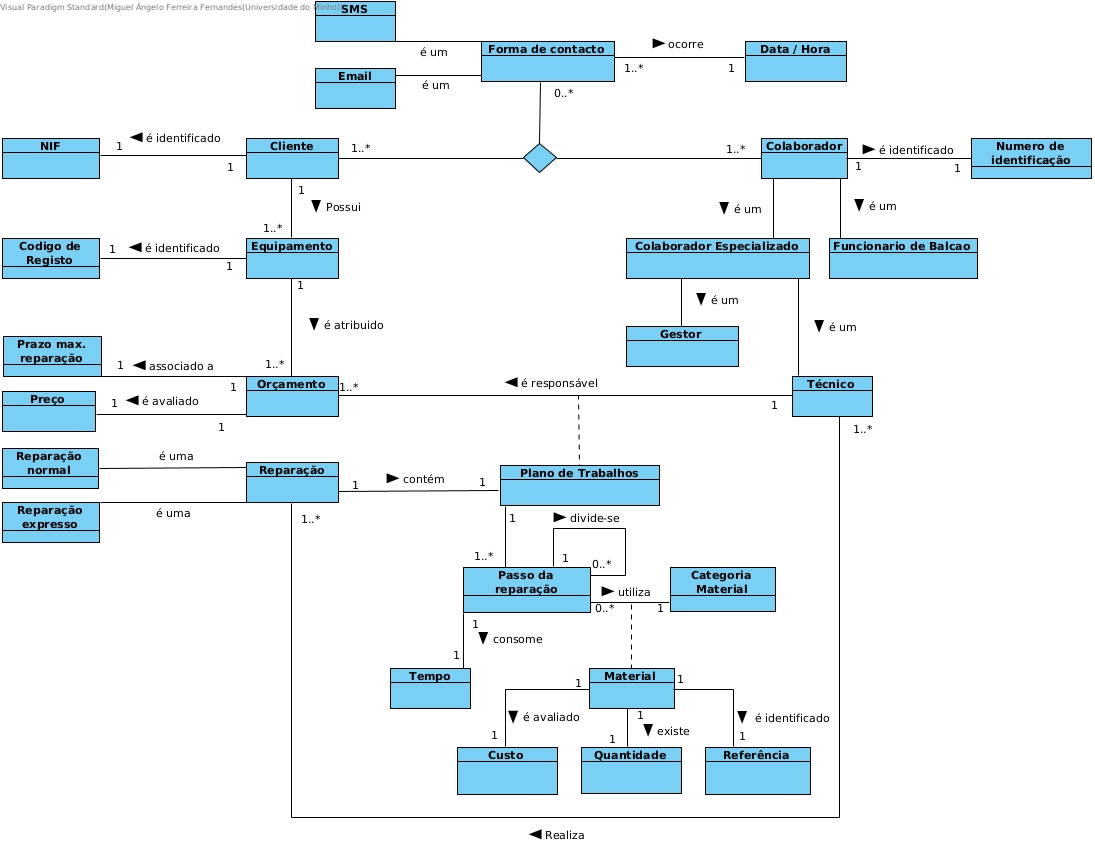
\includegraphics[scale=0.40]{Modelo.jpg}
    \caption{Modelo de Domínio}
\end{figure}

\chapter{Modelação dos Requisitos Funcionais} \label{modelacao_req_funcionais}

A partir dos cenários (ver \ref{cenarios}) identificados pela equipa docente, 
foram identificados os seguintes \textit{use cases}:

\begin{itemize}
    \item Criar reparação expresso - \ref{criar_rep_expresso}
    \item Pedir orçamento - \ref{pedir_orcamento}
    \item Fazer orçamento - \ref{fazer_orcamento}
    \item Criar passo da Reparação - \ref{criar_passo_rep}
    \item Confirmar orçamento - \ref{confirmar_orcamento}
    \item Arquivar orçamento - \ref{arquivar_orcamento}
    \item Realizar reparação - \ref{realizar_rep}
    \item Realizar passo de reparação - \ref{realizar_passo_rep}
    \item Adicionar material - \ref{adicionar_material}
    \item Encomendar material - \ref{encomendar_material}
    \item Receber material - \ref{receber_material}
    \item Entregar equipamento - \ref{entregar_equipamento}
    \item Dar baixo do equipamento - \ref{dar_baixa_equipamento}
    \item Pedir reparação expresso - \ref{pedir_rep_xpress}
    \item Registar equipamento - \ref{registar_equipamento}
    \item Registar cliente - \ref{registar_cliente}
    \item Registar Colaborador - \ref{registar_colab}
    \item Autenticar Colaborador- \ref{autenticar_colab}
    \item Listar resumida do técnico - \ref{listagem_tecnico_resumida}
    \item Listar detalhada do técnico - \ref{listagem_tecnico_detalhada}
    \item Listar funcionário do balcão - \ref{listagem_func_balcao}
\end{itemize}
\section{Modelo de Use Cases}

\begin{figure}
    \centering
    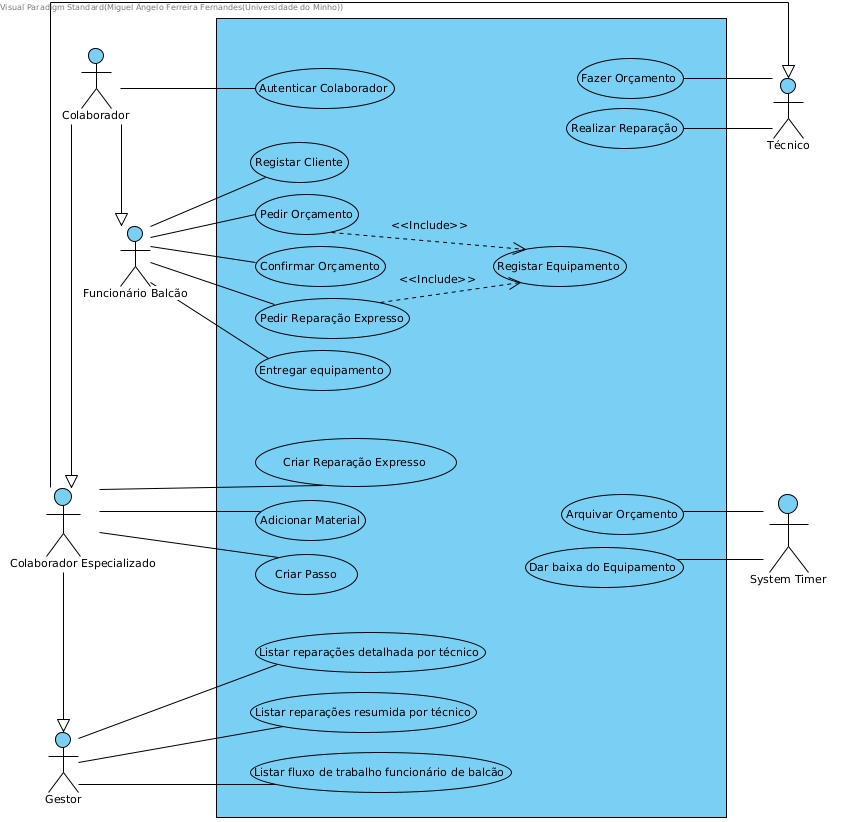
\includegraphics[scale=0.45]{dss-usecase.jpg}
    \caption{Diagrama de \textit{Use Case}}
\end{figure}

\section{Especificação Use Cases}

\subsection{} \label{criar_rep_expresso}
\subfile{use_cases/usecase_criar-rep-xpress.tex}
\noindent{\rule{\textwidth}{0.4pt}

\subsection{} \label{pedir_orcamento}
\subfile{use_cases/usecase_pedir-orcamento.tex}
\noindent{\rule{\textwidth}{0.4pt}

\subsection{} \label{fazer_orcamento}
\subfile{use_cases/usecase_fazer-orcamento.tex}
\noindent{\rule{\textwidth}{0.4pt}

\subsection{} \label{criar_passo_rep}
\subfile{use_cases/usecase_criar-passo.tex}
\noindent{\rule{\textwidth}{0.4pt}

\subsection{} \label{confirmar_orcamento}
\subfile{use_cases/usecase_confirmar-orcamento.tex}
\noindent{\rule{\textwidth}{0.4pt}

\subsection{} \label{arquivar_orcamento}
\subfile{use_cases/usecase_arquivar-orcamento.tex}
\noindent{\rule{\textwidth}{0.4pt}

\subsection{} \label{realizar_rep}
\subfile{use_cases/usecase_realizar-reparacao.tex}
\noindent{\rule{\textwidth}{0.4pt}

\subsection{} \label{realizar_passo_rep}
\subfile{use_cases/usecase_realizar-passo-reparacao.tex}
\noindent{\rule{\textwidth}{0.4pt}

\subsection{} \label{adicionar_material}
\subfile{use_cases/usecase_adicionar-material.tex}
\noindent{\rule{\textwidth}{0.4pt}

\subsection{} \label{encomendar_material}
\subfile{use_cases/usecase_encomendar-material.tex}
\noindent{\rule{\textwidth}{0.4pt}

\subsection{} \label{receber_material}
\subfile{use_cases/usecase_receber-material.tex}
\noindent{\rule{\textwidth}{0.4pt}

\subsection{} \label{entregar_equipamento}
\subfile{use_cases/usecase_entregar-equipamento.tex}
\noindent{\rule{\textwidth}{0.4pt}

\subsection{} \label{dar_baixa_equipamento}
\subfile{use_cases/usecase_dar-baixa.tex}
\noindent{\rule{\textwidth}{0.4pt}

\subsection{} \label{pedir_rep_xpress}
\subfile{use_cases/usecase_pedir-reparacao-expresso.tex}
\noindent{\rule{\textwidth}{0.4pt}

\subsection{} \label{registar_equipamento}
\subfile{use_cases/usecase_registar-equipamento.tex}
\noindent{\rule{\textwidth}{0.4pt}

\subsection{} \label{registar_cliente}
\subfile{use_cases/usecase_registar-cliente.tex}
\noindent{\rule{\textwidth}{0.4pt}

\subsection{} \label{registar_colab}
\subfile{use_cases/usecase_registar-colaborador.tex}
\noindent{\rule{\textwidth}{0.4pt}

\subsection{} \label{autenticar_colab}
\subfile{use_cases/usecase_autenticar-colaborador.tex}
\noindent{\rule{\textwidth}{0.4pt}

\subsection{} \label{listagem_tecnico_resumida}
\subfile{use_cases/usecase_listar-tecnico-resumida.tex}
\noindent{\rule{\textwidth}{0.4pt}

\subsection{} \label{listagem_tecnico_detalhada}
\subfile{use_cases/usecase_listar-tecnico-detalhada.tex}
\noindent{\rule{\textwidth}{0.4pt}

\subsection{} \label{listagem_func_balcao}
\subfile{use_cases/usecase_listar-func-balcao.tex}
\noindent{\rule{\textwidth}{0.4pt}

\chapter{Considerações Finais}
% análise crítica dos resultados

%==========================================================================
% BEGIN LISTA DE SIGLAS E ACRÓNIMOS
%==========================================================================

%% Portuguese babel does not translate this environment
\renewcommand{\nomname}{Lista de Siglas e Acrónimos}

%% Text that can be shown before acronyms list
\renewcommand{\nompreamble}{<<Apresentar uma lista com todas as siglas e acrónimos utilizados durante a realização do trabalho. O formato base para esta lista deverá ser da forma como abaixo se apresenta.>>}

%% acronyms
\nomenclature[01]{\textbf{NIF}}{Número de Idenficação Fiscal}
\nomenclature[02]{UC}{Unidade Curricular}
\nomenclature[03]{DSS}{Desenvolvimento de Sistemas de Software}
\nomenclature[04]{aplicação}{Sistema de Gestão para Centro de Reparação de Equipamento Eletrónico}

%% Show acronyms
\printnomenclature

%==========================================================================
% END LISTA DE SIGLAS E ACRÓNIMOS
%==========================================================================


%==========================================================================
% BEGIN ANEXOS
%==========================================================================

\addchap{Anexos}
\addsec{Anexo 1 - Cenários } \label{cenarios}
\subfile{scenarios/scenario_1.tex}
\subfile{scenarios/scenario_2.tex}
\subfile{scenarios/scenario_3.tex}
\subfile{scenarios/scenario_4.tex}
\subfile{scenarios/scenario_5.tex}

%==========================================================================
% END ANEXOS
%==========================================================================


\end{document}